\documentclass[12pt]{article}
\usepackage{graphicx}
\usepackage{amssymb}

\begin{document}

\section*{Set Theory}
\Large
\begin{itemize}
\item[1.1] Introduction  
\item[1.2] Sets  
\item[1.3] Sub-sets  
\item[1.4] The order of sets: finite and infinite sets .
\item[1.5] Union and intersection of sets  
\item[1.6] Differences and complements  
\item[1.7] Venn diagrams  
\item[1.8] Logic analysis
\end{itemize}  
%-----------------------------------------------------%
\newpage
\subsection*{Union and intersection of sets}

\begin{itemize}
\item The \textbf{union} of two sets A and B is a set containing all the elements in
either A or B (or both)
i.e. 
\[A \cup B = {x / x \in A \mbox{ or } x \in B}.\]
\item The \textbf{intersection} of two sets A and B is a set containing all the elements
that are both in A and B
i.e. 
\[A \cap B = {x / x \in A \mbox{ and }x \in B}\].

\item If sets A and B have no elements in common, i.e. $A \cap B = \emptyset$,then A and B
are termed \textbf{disjoint sets}.
\end{itemize}
\newpage
\subsection*{Subsets}

\begin{itemize}
\item Proper Subsets
\end{itemize}
\subsection*{The Power Set}

\newpage
\subsection*{Venn Diagrams}
\begin{figure}
\centering
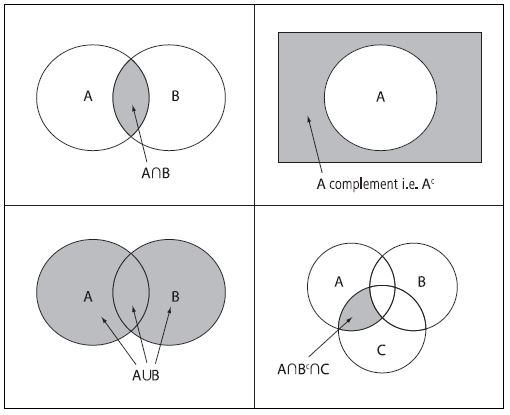
\includegraphics[width=0.7\linewidth]{venndiagram}

\end{figure}

\end{document}


